\chapter{Az üzleti folyamatok elemeinek leképzése}

%TODO Ide kellene felsorolni, és részletesen leírni, hogy a BPEL egyes elemeinek milyen Petri-háló feleltethető meg.

%TODO Megnézni, hogy az egyes elemek esetében milyen alternatívák lennének a leképzésre!
\section{A leképzés menete}
A BPEL nyelv az egymással együttműködő modulok működését szimulálja. A BPEL  modellben a folyamat lépéseit tevékenységnek \textsl{activity} nevezzük. A tevékenységek lehetnek elemiek és összetettek. Tipikus elemi tevékenységek:
\begin{itemize}
\item más funkció meghívása,
\item üzenet küldés/fogadás,
\item változók módosítása,
\item várakozás, szinkronizálás.
\end{itemize}
Az elemi tevékenységekből összetett folyamatok építhetőek fel szekvencia, párhuzamosítás és ciklus elemek segítségével.

A BPEL szabvány tevékenység készletének bemutatásánál csak a legfontosabb elemekre térünk most ki. A szabvány részletei a
http://docs.oasis-open.org/wsbpel/2.0/OS/wsbpel-v2.0-OS.html weboldalról érhetőek el. 

A BPEL definíció egyértelműsíti a folyamat kezdetét és inicializálja is a megfelelő paraméterekkel. A Petri háló erre nem tér ki, ezért bevezetünk egy opcionális \textit{START} tranazíciót. Ennek feladata, a megfelelő tokenek legenerálása a folyamat indításához. A folyamat zárása szintén egyértelmű a BPEL szabványban. Petri háló kapcsán beszélhetünk a háló leállásáról, ha már semmilyen hely és tranzíció nem produkál új tokent, nem várakozik és nem nyel el tokent. A köztes elemek leképzése általánosan nem bonyolult, de megvizsgálhatók alternatív leképzési módok. 

Az alkalmazás jelölésrendszere: A rendszer a helyeket P-vel, míg a tranzíciókat T-vel indexeli. A helyek után listázza az adott helyen levő tokeneket. A jelenleg lépésben levő tranzíciók pedig színes kitöltést kapnak.

\section{\texttt{<receive>}}

Egy megfelelő üzenet után engedi a folyamatot továbbhaladni, így várakoztatáshoz használható. A \texttt{<receive>} típusú XML elemekhez tartozó sémaleírás:\\
\begin{verbatim}
<receive partnerLink="NCName"
   portType="QName"?
   operation="NCName"
   variable="BPELVariableName"?
   messageExchange="NCName"?>
   <fromParts>?
      <fromPart part="NCName" toVariable="BPELVariableNm"/>+
   </fromParts>
</receive>
\end{verbatim}
A hálóban ezt egy tranzicióval könnyedén megoldhatjuk, hiszen csak egy specifikus üzenet token kell a továbblépéshez, és a többit addig az előző helyen parkoltatja. 

\section{\texttt{<reply>}}
Üzenetküldő elem, ami \texttt{<receive>; <onMessage>;<onEvent>} események után léphet akcióba. 
\begin{verbatim}
<reply partnerLink="NCName"
   portType="QName"?
   operation="NCName"
   variable="BPELVariableName"?
   messageExchange="NCName"?>
   <toParts>?
      <toPart part="NCName" fromVariable="BPELVariableNm"/>+
   </toParts>
</reply>
\end{verbatim}
A lekezelése az előző példával analóg módon, annyi különbséggel, hogy a tokenek nem parkolnak, hanem tovább mennek és a tranzíció csak akkor generál új tokent ha üzenetet kap egy ágról.

\section{\texttt{<invoke>}}
Egy BPEL vagy épp egy webszolgáltatás meghívására szolgál és definiálja a szolgáltatás feladatát is. 
\begin{verbatim}
<invoke partnerLink="NCName"
   portType="QName"?
   operation="NCName"
   inputVariable="BPELVariableName"?
   outputVariable="BPELVariableName"?>
   <catch faultName="QName"? … >*
  	activity
   </catch>
   <toParts>?
      <toPart part="NCName" fromVariable="BPELVariableNm"/>+
   </toParts>
   <fromParts>?
      <fromPart part="NCName" toVariable="BPELVariableNm"/>+
   </fromParts>
</invoke>
\end{verbatim}
A grafikus megjelenítése \aref{fig:invoke}. ábrán látható.

\begin{figure}[h!]
\centering
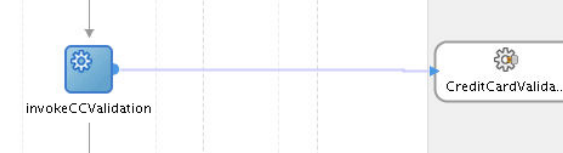
\includegraphics[scale=0.6]{images/invoke.png}
\caption{Az \texttt{invoke} grafikus jelölése az Oracle BPEL designer-ben}
\label{fig:invoke}
\end{figure}

Használatát a programrészek újrafelhasználhatósága indokolja, valamint az átláthatósági alapelvek. Például, az ábrán látható CCvalidation használható ATM-es pénz felvét, egyenleglekérdezés, vagy egyéb ATM nél végezhető művelet során. 

\begin{figure}[h!]
\centering
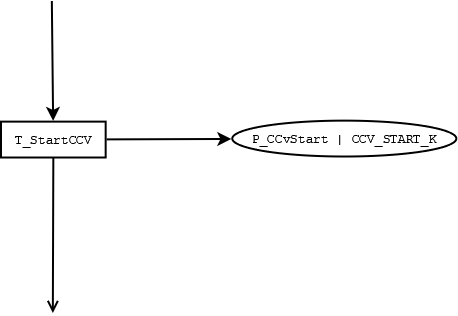
\includegraphics[scale=0.4]{images/invokenet.png}
\caption{Az \texttt{<invoke>} leképzése petri hálóra}
\label{fig:invokenet}
\end{figure}
Leképzés során ügyelni kell arra, hogy az \texttt{invoke} paramétereinek megfelelő tokenek keletkezzenek és legyenek átadva a részháló start elemének.

\section{\texttt{<assign>}}

Egy változó értékadására szolgáló esemény. Ellentétben egy imperatív értékadással egy \texttt{<assign>} blokkban bármennyi értékadás, másolás történhet, amíg azt a kliens kezelni tudja, így logikailag egy egységbe zárja a műveleteket.  
\begin{verbatim}
<assign validate="yes|no"? standard-attributes>
   (
   <copy keepSrcElementName="yes|no"? 
  	from-spec
  	to-spec
   </copy>
</assign>
\end{verbatim}
Az érték hozzárendelése nagyon egszerűen átírható egy tranzicióra ami a megfelelő tokenek színét módosítja. 
A grafikus megjelenítése \aref{fig:assign}. ábrán látható.
A színmódosítás egyszerűen a token nevének átírását jelenti. 
\begin{figure}[h!]
\centering
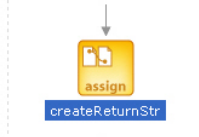
\includegraphics[scale=1]{images/assign.png}
\caption{Az \texttt{assign} grafikus jelölése az Oracle BPEL designer-ben}
\label{fig:assign}
\end{figure}

\begin{figure}[h!]
\centering
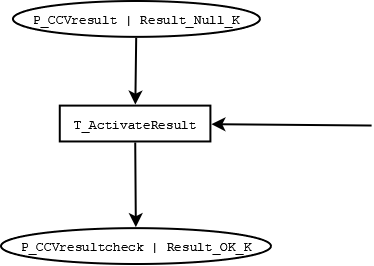
\includegraphics[scale=0.4]{images/assignnet.png}
\caption{Az \texttt{assign} leképzése petri hálóra}
\label{fig:assignnet}
\end{figure}
Az ábrán egy változós értékadásra látható példa. Hasonló módon kezelendő a  blokkosított értékadás, a különbség, hogy a több token jöhet és távozhat több forrásba is.

\section{\texttt{<validate>}}
Egy sémára validálja az XML (BPEL) állományt. 
\begin{verbatim}
<validate variables="BPELVariableNames" standard-attributes>
   standard-elements
</validate>
\end{verbatim}
Mivel a Petri háló nem tartalmaz validációs elemeket, ezért a \texttt{<validate>} nem képződik le. 

\section{\texttt{<throw>}}
Egy rész processzen belül fault generálására szolgál. 
\begin{verbatim}
<throw faultName="QName"
   faultVariable="BPELVariableName"?
   standard-attributes>
   standard-elements
</throw>
\end{verbatim}
Nagyon egyszerűen egy \textit{fault} tokent generáló tranzició komponens. Explicit hálórésze nincs, hanem a megfelelő inputtokenek megléte vagy hiánya generálja egy tranzició során. 

\section{\texttt{<wait>}}
Időre vonatkoztatva várakoztat. Például 5000 tick vagy 14:00:23 (hh:mm:ss)
\begin{verbatim} 
<wait standard-attributes>
   standard-elements
   (
   <for expressionLanguage="anyURI"?>duration-expr</for>
   |
   <until expressionLanguage="anyURI"?>deadline-expr</until>
   )
</wait>
\end{verbatim}
Megadható egy részhálóval ami valójában egy oszcillátor és a megfelelő iteráció után folytat tokent küld. Továbbá létezik úgynevezett időérzékeny háló, ahol az elemek tokenátadási sebessége ismert, vagy állítható. Ezzel időzítőt lehet létrehozni. Esetenként hardware-es óra is használható

\section{\texttt{<empty>}}
No-op (\textit{no operations}) esemény szinkronizációra szolgál.
\begin{verbatim}
<empty standard-attributes>
   standard-elements
</empty>
\end{verbatim}
Beiktatható egy semleges tranzició és hely.

\section{\texttt{<sequence>}}
Sorozatot ad meg.
\begin{verbatim}
<sequence standard-attributes>
   standard-elements
   activity+
</sequence>
\end{verbatim}
Egyszerűen csak tranziciók és helyek összefűzése. 

\section{\texttt{<if>}}

\texttt{<if>} Standard kétirányú elágazás. Logikai XPATH kifejezést vár. 
\begin{verbatim}
<if standard-attributes>
   standard-elements
   <condition >bool-expr</condition>
   activity
   <elseif>*
      <condition>bool-expr</condition>
  	activity
   </elseif>
   <else>?
  	activity
   </else>
</if>
\end{verbatim}
Egy tranzició, mely tokenek függvényében más felé küldi tovább, vagy generál tokeneket. Ez lehet egy helyen összegyúlt tokenek mennyisége, vagy egy adott helyen egy specifikus színű token megléte, vagy nemléte. Analóg módon egy \textit{Switch-Case} elágazás is definiálható vele.
A PBEL-es grafikus megjelenítése \aref{fig:if}. ábrán látható.

\begin{figure}[h!]
\centering
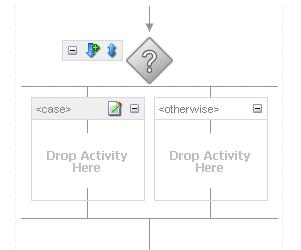
\includegraphics[scale=1]{images/if.png}
\caption{Az \texttt{if} grafikus jelölése az Oracle BPEL designer-ben}
\label{fig:if}
\end{figure}


\begin{figure}[h!]
\centering
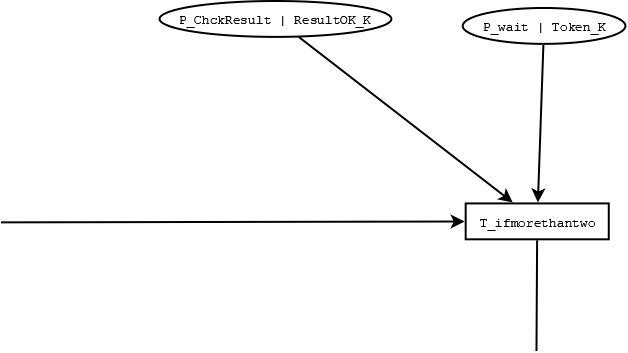
\includegraphics[scale=0.4]{images/ifnet.png}
\caption{Az \texttt{if} Egy hálóképzése}
\label{fig:ifnet}
\end{figure}

\section{\texttt{<while>}}
Elöltesztelős ciklus. Addig iterál, amíg az ciklus feltétel igaznak értékelődik ki. 
\begin{verbatim}
<while standard-attributes>
   <condition>bool-expr</condition>
   activity
</while>
\end{verbatim}
Egy tranzició, mely token függvényében a folyamat egy korábbi pontjára csatol vissza, vagy éppen egy későbbire, a feltétel hamis logikai állapota esetén. A feltétel persze egy színes token jelenléte, vagy tokenek száma is lehet. 

\section{\texttt{<repeatUntil>}}
Egy hátultesztelős ciklusnak feleltethető meg, amely akkor enged tovább, ha a feltétel igaz. 
\begin{verbatim}
<repeatUntil standard-attributes>
   standard-elements
   activity
   <condition expressionLanguage="anyURI"?>bool-expr</condition>
</repeatUntil>
\end{verbatim}
A \texttt{<while>}-al analóg módon megadható a Petri-hálós leképzése.

\section{\texttt{<forEach>}}
Végig iterál a gyerekelemeken. Megadható párhuzamos feldolgozás is. Egy \textit{Complete condition} segítségével megadható egy break utasítás ami kilép a ciklusból. 
\begin{verbatim}
<forEach counterName="BPELVariableName" parallel="yes|no">
   <startCounterValue expressionLanguage="anyURI"?>
  	unsigned-integer-expression
   </startCounterValue>
   <finalCounterValue expressionLanguage="anyURI"?>
  	unsigned-integer-expression
   </finalCounterValue>
</forEach>
\end{verbatim}
Egyszerű loop utasítás, azonban párhuzamosítás esetén a részhálóból megfelelő példányszámot generáltatunk. 

\section{\texttt{<pick>}}
Üzenetek várására vagy időtúllépés eseményre figyel. Ezek bármelyike a szubprocessz végrehajtásához vezet. 
\begin{verbatim}
<pick createInstance="yes|no"? standard-attributes>
   standard-elements
   <onMessage partnerLink="NCName"
      portType="QName"?
      operation="NCName"
      variable="BPELVariableName"?
      messageExchange="NCName"?>+
      <correlations>?
         <correlation set="NCName" initiate="yes|join|no"? />+
      </correlations>
      <fromParts>?
         <fromPart part="NCName" toVariable="BPELVariableName" />+
      </fromParts>
      activity
   </onMessage>
   <onAlarm>*
      (
      <for expressionLanguage="anyURI"?>duration-expr</for>
      |
      <until expressionLanguage="anyURI"?>deadline-expr</until>
      )
      activity
   </onAlarm>
</pick>
\end{verbatim}
A grafikus megjelenítése \aref{fig:pick}. ábrán látható.

\begin{figure}[h!]
\centering
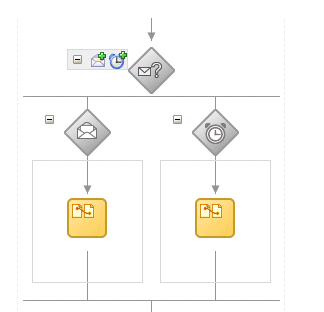
\includegraphics[scale=1]{images/pick.png}
\caption{A \texttt{pick} grafikus jelölése az Oracle BPEL designer-ben}
\label{fig:pick}
\end{figure}

Összetartó hálóval és egy tranzícióval képezhető le.


\section{\texttt{<flow>}}

Konkurens elemek deklarálására szolgál. Linkek segítségével megadható függőségi viszony a gyerekek között. 
\begin{verbatim}
<flow standard-attributes>
   standard-elements
   <links>?
      <link name="NCName" />+
   </links>
   activity+
</flow>
\end{verbatim} 
A grafikus megjelenítése \aref{fig:flow}. ábrán látható.

\begin{figure}[h!]
\centering
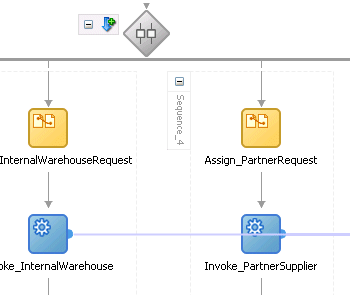
\includegraphics[scale=1]{images/flow.png}
\caption{A \texttt{flow} grafikus jelölése az Oracle BPEL designer-ben}
\label{fig:flow}
\end{figure}
Leképzése egyszerű, hisz a megfelelő gyerek elemek nem szekvenciálisan helyezkednek el, hanem párhuzamosan.
\section{\texttt{<scope>}}

A gyerek elemek hatókörét lehet vele szabályozni.
\begin{verbatim}
<scope isolated="yes|no"? exitOnStandardFault="yes|no"?
   standard-attributes>
   standard-elements
   <partnerLinks>?
      ... see above under <process> for syntax ...
   </partnerLinks>
   <messageExchanges>?
      ... see above under <process> for syntax ...
   </messageExchanges>
   <variables>?
      ... see above under <process> for syntax ...
   </variables>
   <correlationSets>?
      ... see above under <process> for syntax ...
   </correlationSets>
   <faultHandlers>?
      ... see above under <process> for syntax ...
   </faultHandlers>
   <compensationHandler>?
      ...
   </compensationHandler>
   <terminationHandler>?
      ...
   </terminationHandler>
   <eventHandlers>?
      ... see above under <process> for syntax ...
   </eventHandlers>
   activity
</scope>
\end{verbatim}
Nem generál új elemet, csak a láthatósági, azaz visszacsatolási elemeket adja meg. 


